\section*{Microeconomics Midterm 2016 / 17 (1)}

There are somehow two midterms for this year. This is one of the exams.

{
\subsection*{Schmidt}

\subsubsection*{Exercise 1}

\begin{enumerate}[label=(\alph*)]
{\item 
Use Roy's identity on some monotonic transformation $f(\cdot)$ of $v(p, w)$ :

$$
\begin{aligned}
\tilde{x}_{l}(p, w) & =-\frac{\frac{\partial f(v(p, w))}{\partial p_{l}}}{\frac{\partial f(v(p) w)}{\partial w}}=-\frac{\frac{\partial f(v(p, w))}{\partial v(p, w)} \cdot \frac{\partial v(p, w)}{\partial p_{l}}}{\frac{\partial f(p(p, w))}{\partial v(p, w)} \cdot \frac{\partial v(p, w)}{\partial w}} \\
& =-\frac{\frac{\partial v(p, w)}{\partial p_{l}}}{\frac{\partial v(p, w)}{\partial w}}=x_{l}(p, w)
\end{aligned}
$$
}
{\item 
(1) invert $v(p, w)$ to obtain e(p,u). In equilibrium

$$
\begin{aligned}
& v\left(p_{1}, w\right)=u \quad ; \quad e\left(p_{1}, u\right)=w \\
& u=\left(\frac{\alpha}{p_{1}}\right)^{\alpha}\left(\frac{1-\alpha}{p_{2}}\right)^{1-\alpha} e\left(p_{1}, u\right) \\
& \Leftrightarrow \quad e\left(p_{1}, u\right)=u\left(\frac{p_{1}}{\alpha}\right)^{\alpha}\left(\frac{p_{2}}{1-\alpha}\right)^{1-\alpha}
\end{aligned}
$$

(2) Apply Shepherd's Lemma:

$$
\begin{aligned}
h_{1}\left(p_{1}, u\right) & =\frac{\partial e\left(p_{1} u\right)}{\partial p_{1}}=u\left(\frac{p_{2}}{1-\alpha}\right)^{1-\alpha}\left(\frac{1}{\alpha}\right)^{\alpha} k p_{1}^{\alpha-1} \\
& =u\left(\frac{p_{2} \alpha}{(1-\alpha) p_{1}}\right)^{1-\alpha}
\end{aligned}
$$
}
{\item 
\underline{case 1:}

$$
\begin{aligned}
& \alpha=\alpha\left(p_{1} / p_{2}\right) \longrightarrow \alpha\left(\lambda p_{1} / \lambda p_{2}\right)=\alpha\left(p_{1} / p_{2}\right) \\
& h_{1}\left(\lambda p_{1}, u\right)=u\left(\frac{\lambda p_{2} \alpha\left(p_{1} / p_{2}\right)}{\left(1-\alpha\left(p_{1} / p_{2}\right)\right) \lambda p_{1}}\right)^{1-\alpha\left(p_{1} / p_{2}\right)} \\
&=u\left(\frac{p_{2} \alpha\left(p_{1} / p_{2}\right)}{\left(1-\alpha\left(p_{1} / p_{2}\right)\right) p_{1}}\right)^{1-\alpha\left(p_{1} / p_{2}\right)}=h_{1}\left(p_{1},  u\right)
\end{aligned}
$$

\underline{case 2:}
 $\alpha=\alpha\left(p_{1}\right) \longrightarrow \alpha\left(\lambda p_{1}\right) \neq \alpha\left(p_{1}\right)$

$$
\begin{aligned}
h_{1}\left(\lambda p_{1}, u\right) & =u\left(\frac{\lambda p_{2} \alpha\left(\lambda p_{1}\right)}{\left(1-\alpha\left(\lambda p_{1}\right)\right) \lambda p_{1}}\right)^{1-\alpha\left(\lambda p_{1}\right)} \\
& =u\left(\frac{p_{2} \alpha\left(\lambda p_{1}\right)}{\left(1-\alpha\left(\lambda p_{1}\right)\right) p_{1}}\right)^{1-\alpha\left(\lambda p_{1}\right)} \neq h_{1}\left(p_{1}, u\right)
\end{aligned}
$$
}
\end{enumerate}
}
{
\subsubsection*{Exercise 2}

$$
A=-E V\quad ; \quad B=-C V
$$

Note that we can transform $U\left(x_{1}, x_{2}\right)$ to have Cobb-Douglas:

$$
\tilde{u}\left(x_{1}, x_{2}\right)=\left(x_{1} x_{2}\right)^{1 / 2}
$$

Thus:

$$
\begin{aligned}
& x_{1}(p, w)=\frac{1}{2} \frac{w}{p_{1}} ; x_{2}(p, w)=\frac{1}{2} \frac{w}{p} \\
& v(p, w)=\frac{w}{2}\left(\frac{1}{p_{1} p_{2}}\right)^{1 / 2}
\end{aligned}
$$

Before moving:

$$
v_{0}(p, w)=\frac{3000}{2}=1500
$$

After moving (no raise):

$$
v_{1}(p, w)=\frac{3000}{2}\left(\frac{1}{2.25}\right)^{1 / 2}=1000
$$

Calculate A by subtracting from $w$ and let $p_{1}=p_{2}=1$.

Same utility as after move without raise:

$$
\begin{aligned}
& & v_{1}(p, w) & =\frac{w-A}{2} \\
& & 1000 & =\frac{3000-A}{2} \\
& & A & =1000
\end{aligned}
$$

Calculate $B$ by adding to $w$ letting $p_{1}=1, p_{2}=2.25$.

same utility as before moving:

$$
\begin{aligned}
v_{0}(p, w) & =\frac{w+B}{2}\left(\frac{1}{p_{1} p_{2}}\right)^{1 / 2} \\
1500 & =\frac{3000+B}{2}\left(\frac{1}{2.25}\right)^{1 / 2} \\
B & =1500
\end{aligned}
$$
}
{\subsubsection*{Exercise 3}
\begin{enumerate}[label=(\alph*)]
{\item 
(1) Solve CMP for $f(x)=1$ :

\begin{align*}
    \min _{x} w x \\
    \text{s.t. } f(x)=1
\end{align*}

First order conditions:

\begin{align*}
    w_{l}-\lambda \frac{\partial f(x)}{\partial x_{l}}=0 \quad \forall l & \mid \cdot x_{l} \\
    w_l x_l -\lambda \frac{\partial f(x)}{\partial x_{l}} x_{l}=0 \quad \forall l & \mid \text{ sum over } l \\
    \sum_{l} w_{l} x_{l}-\lambda \sum_{l} \frac{\partial f(x)}{\partial x_{l}} x_{l}=0 & \\
    w x=\lambda \sum_{l} \frac{f(x)}{\partial x_{l}} x_{l} & \mid \text{ by CRS apply Euler} \\
    w x=\lambda f(x) & \mid \text{ use } f(x) = 1 \\
    w x=\lambda=c(w) & 
\end{align*}

(2) Solve CMP for $f(x)=y$ :

\begin{align*}
    \min _{x} w x \\
    \text{s.t. } f(x)=y
\end{align*}

Up to $w x=\lambda f(x)$ everything is identical:

$$
\begin{aligned}
& w x=\lambda f(x) \quad \mid \text { use } f(x)=y \\
& w x=\lambda y=c(w, y)=c(w) \cdot y
\end{aligned}
$$
}
{\item 
Apply Shephard's Lemma:

$$
\begin{aligned}
& x_{l}(w)=\frac{\partial c(w)}{\partial w_{l}} \\
& x_{l}(w, y)=\frac{\partial c(w, y)}{\partial w_{l}}=y \frac{\partial c(w)}{\partial w_{l}}=y \cdot x_{l}(w)
\end{aligned}
$$
}
{\item 
Profits are

$$
\begin{aligned}
\pi & =p f(x)-w x \\
& =p f(x)-\sum_{l} p \frac{\partial f(x)}{\partial x_{l}} x_{l} \\
& =p\left[f(x)-\sum_{l} \frac{\partial f(x)}{\partial x_{l}} x_{l}\right]
\end{aligned}
$$

By Euler \& CRS we know that

$$
\sum_{l} \frac{\partial f(x)}{\partial x_{l}} x_{l}=f(x)
$$

Thus :

$$
\pi=p\left[f(x)-\sum_{l} \frac{\partial f(x)}{\partial x_{l}} x_{l}\right]=0
$$
}
\end{enumerate}
}
\newpage
{
\subsection*{Gottardi}

\subsubsection*{Exercise 1}

\begin{enumerate}[label=(\alph*)]
{\item 
For $A$ must have $x_{1}^{A}=x_{2}^{A}$ while $B$ is happy with having only one good. Easiest to look at it in Edgeworth box:

\begin{figure}[!htp]
    \centering
    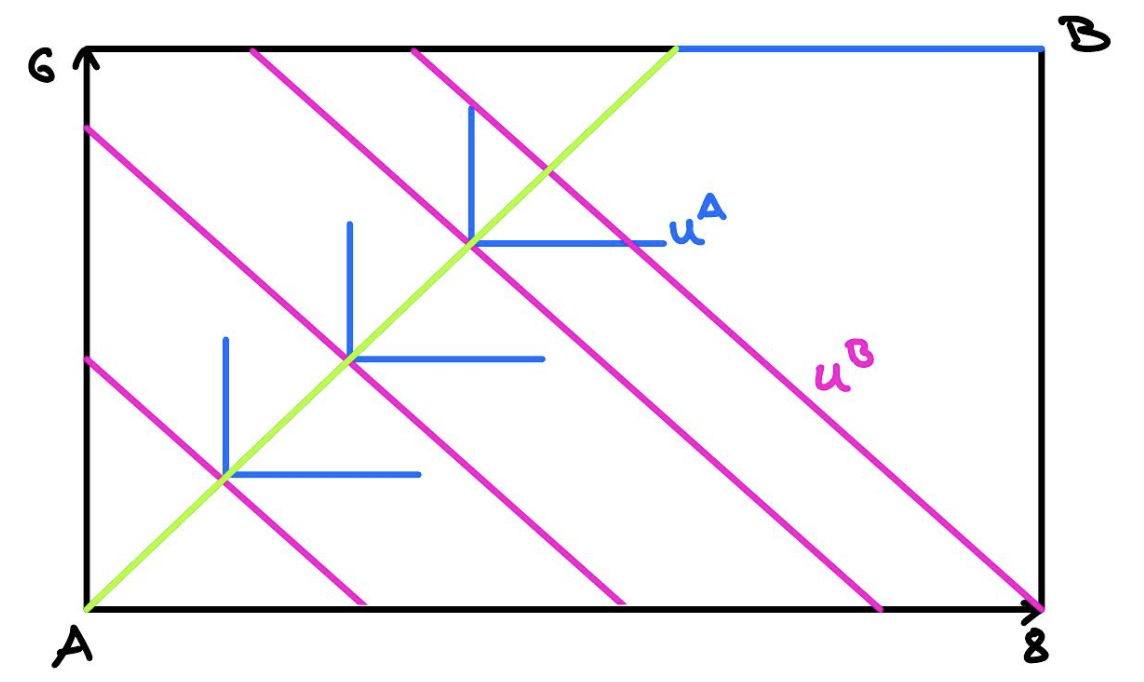
\includegraphics[width=.75\textwidth]{images/2016_17_1_1.png}
\end{figure}

Look at ind. curves to see that only PE allocations are on $x_{1}^{A}=x_{2}^{A}$ as long os $x_{1}^{A}<6$ Green or PE.

If $u^{A}\left(x_{1}^{A}, x_{2}^{A}\right)=x_{1}^{A}+2 x_{2}^{A}$ wed have the following Edgeworth Box:

\begin{figure}[!htp]
    \centering
    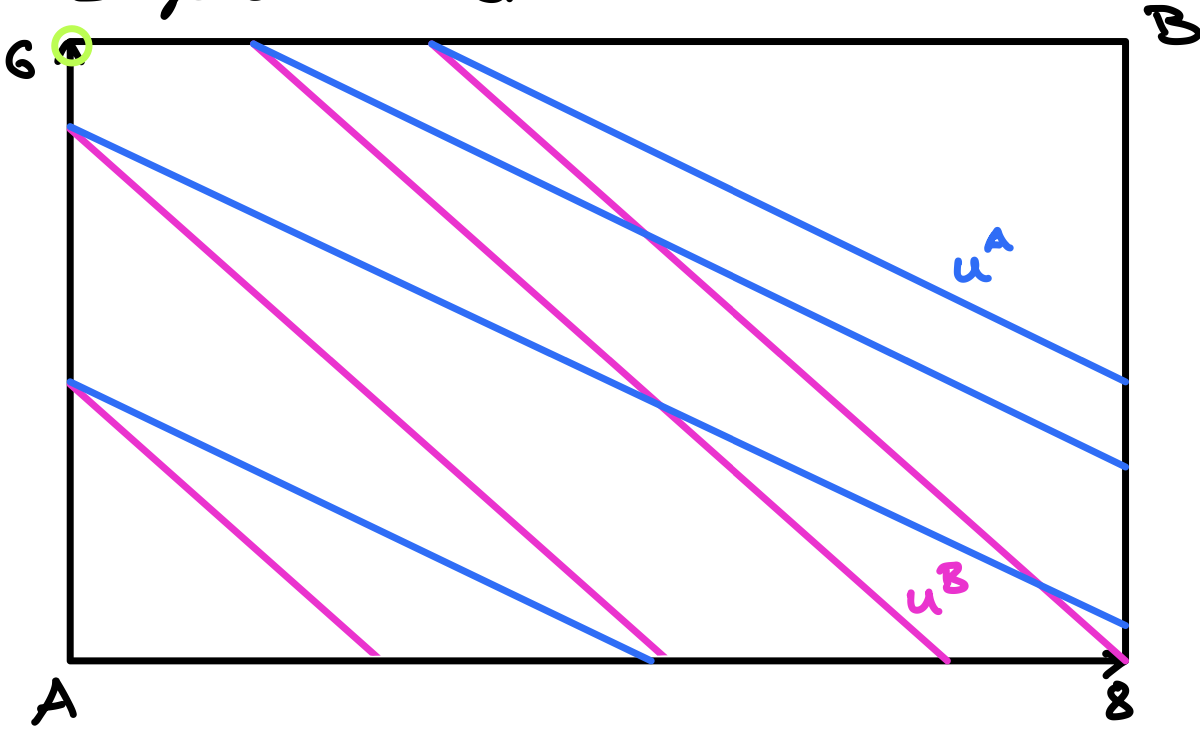
\includegraphics[width=.75\textwidth]{images/2016_17_1_2.png}
\end{figure}

Only PE allocation is the top left corner. As A values $x_{2}$ more, she gets all of it.
}
{\item 
Let $p=p_{1} / p_{2}$.

consumer A: Leontief implies $x_{1}^{A}=x_{2}^{A}$

consumer $B$ : This is Cobb-Douglas with $\alpha=1 / 2$. Thus:

$$
x_{2}^{8}=\frac{6}{2}=3 \text { and } x_{1}^{B}=\frac{6}{2 p}=\frac{3}{p}
$$
markets: $\quad x_{1}^{A}+x_{1}^{B}=6 \Leftrightarrow x_{1}^{A}=3$

Use this in $x_{1}^{A}=x_{2}^{A}: \quad x_{2}^{A}=3$

$$
x_{2}^{A}+x_{2}^{B}=8 \Longleftrightarrow x_{2}^{B}=5
$$

Determine price:

$$
x_{2}^{B}=3 / p \Leftrightarrow p=3 / 5
$$

\underline{Competitive Equilibrium:}

$$
\begin{aligned}
\left(x_{1}^{A}, x_{2}^{A}\right) & =(3,3) \\
\left(x_{1}^{B}, x_{2}^{3}\right) & =(3,5) \\
p & =3 / 5
\end{aligned}
$$
}
{\item 
Look at excess demand:

$$
\begin{aligned}
z_{1} & =x_{1}^{A}+x_{1}^{B}-w_{1}^{A}=x_{1}^{A}+\frac{3}{p_{1}}-8 \\
\frac{\partial z_{1}}{\partial p_{1}} & =-\frac{3}{p_{1}^{2}}<0 \\
z_{2} & =x_{2}^{A}+x_{2}^{B}-w_{2}^{B}=x_{2}^{A}+\frac{3}{p_{2}}-6 \\
\frac{\partial z_{2}}{\partial p_{2}} & =-\frac{3}{p_{2}^{2}}<0
\end{aligned}
$$

Excess demand is upward sloping, thus the CE is unique.

It is PE by FWT. We have LNS of preferences, complete markets, and free disposal.
}
\end{enumerate}
}
{
\subsubsection*{Exercise 2}
$$
w^{A}=(12,2) \quad w^{B}=(2,8)
$$
\begin{enumerate}[label=(\alph*)]
{\item
for either consumer $h \in\{A, B\}$

at $t=0$ :

$$
q_{1} \theta_{1}^{h}+q_{2} \theta_{2}^{h}=0
$$

at $t=1$:

$$
\begin{aligned}
& x_{1}^{h}=\theta_{1}^{h}+w_{1}^{h} \\
& x_{2}^{h}=\theta_{2}^{h}+w_{2}^{h}
\end{aligned}
$$

Together:

$$
q_{1}\left(x_{1}^{h}-w_{1}^{h}\right)+q_{2}\left(x_{2}^{h}-w_{2}^{h}\right)=0
$$
}
{\item 
\underline{consumer h:}

$$
\begin{gathered}
\max _{x_{1}^h, x_{2}^{h}} \pi_{1}^{h} u^{h}\left(x_{1}^{h}\right)+\pi_{2}^{h} u^{h}\left(x_{2}^{h}\right) \\
\text { s.t. } q_{1}\left(x_{1}^{h}-w_{1}^{h}\right)+q_{2}\left(x_{2}^{h}-w_{2}^{h}\right)=0
\end{gathered}
$$

FOCs:

$$
\begin{gathered}
\left[x_{1}^{h}\right]: \pi_{1}^{h} \frac{\partial u^{h}\left(x_{1}^{h}\right)}{\partial x_{1}^{h}}-\lambda q_{1}=0 \\
{\left[x_{2}^{h}\right]: \pi_{2}^{h} \frac{\partial u^{h}\left(x_{2}^{h}\right)}{\partial x_{2}^{h}}-\lambda q_{2}=0}
\end{gathered}
$$

Note that by risk-neutrality of $A$, we have $\frac{\partial u^{A}(.)}{\partial x_{2}^{A}}=1$ :

$$
\frac{q_{1}}{q_{2}}=\frac{\pi_{1}^{A}}{\pi_{2}^{A}}=1
$$

If we plug this into the FOCs for $B$, we obtain:

$$
\begin{aligned}
& 1=\frac{q_{1}}{q_{2}}=\frac{\pi_{1}^{B} \frac{\partial u^{B}\left(x_{1}^{B}\right)}{\partial x_{1}^{B}}}{\pi_{2}^{B} \frac{\partial u^{B}\left(x^{B}\right)}{\partial x_{2}^{B}}}=\frac{\frac{\partial u^{B}\left(x_{1}^{B}\right)}{\partial x_{1}^{B}}}{\frac{\partial u^{B}\left(x^{B}\right)}{\partial x_{2}^{B}}} \\
& \Leftrightarrow \frac{\partial u\left(x_{1}^{B}\right)}{\partial x_{1}^{B}}=\frac{\partial u\left(x^{B}\right)}{\partial x_{2}^{B}} \\
& \Leftrightarrow x_{1}^{B}=x_{2}^{B}
\end{aligned}
$$

Plug this into $B C$ for $B$ :

$$
\begin{aligned}
\frac{q_1}{q_2}\left(x_{1}^{B}-w_{1}^{B}\right)+\left(x_{2}^{B}-w_{2}^{B}\right) & =0 \\
x_{1}^{B}-2+x_{1}^{B}-8 & =0 \\
x_{1}^{B} & =5=x_{2}^{B}
\end{aligned}
$$

\underline{markets:}

$$
\begin{aligned}
& x_{1}^{A}+x_{1}^{B}=14 \Rightarrow x_{1}^{A}=9 \\
& x_{2}^{A}+x_{2}^{B}=10 \Rightarrow x_{2}^{A}=5
\end{aligned}
$$

\underline{Competitive Equilibrium:}

$$
\begin{array}{ll}
& \left(x_{1}^{A}, x_{2}^{A}\right)=(9,5) \\
& \left(x_{1}^{B}, x_{2}^{B}\right)=(5,5)
\end{array} \quad \frac{q_{1}}{q_{2}}=1
$$

Due to risk neutrality of $A$, she carries all the risk while B perfectly smooths her consumption. At the same time this implies that A's beliefs determine the price ratio of the securities. By $\pi_{1}^{A}=\pi_{2}^{A}$ we have $q_{1}=q_{2}$.
}
{\item 
No. The prices will change as they reflect A's beliefs:

$$
\frac{q_{1}}{q_{2}}=\frac{\pi_{1}^{A}}{\pi_{2}^{A}}>1
$$

Use B's budget constraint: (sill $x_{1}^{B}=x_{2}^{B}$ )

$$
\begin{aligned}
& q_{1}\left(x_{1}^{B}-2\right)+q_{2}\left(x_{1}^{B}-8\right)=0 \\
& x_{1}^{B}\left(q_{1}+q_{2}\right)=2 q_{1}+8 q_{2} \\
& x_{1}^{B}=\frac{2 q_{1}+8 q_{2}}{q_{1}+q_{2}}=\frac{2\frac{q_1}{q_{2}}+8}{1+q_{1}/ q_{2}} \\
& \frac{\partial x_{1}^{B}}{\partial q_{1}/ q_{2}}=\frac{2\left(1+q_{1}/ q_{2}\right)-\left(2 q_{1}/ q_{2}+8\right)}{\left(1+q_{1}/ q_{2}\right)^{2}}=\frac{-6}{\left(1+q_{1}/q_{2}\right)^{2}}<0
\end{aligned}
$$

We see that $B$ consumes less which makes sense as the asset that would insure her against her poor state $(s=1)$ has become more expensive \& she purchases less of it.

By market clearing, A consumes more.
}
\end{enumerate}
}
